%%=====================================================================
%% Detecting Purpose-Code Gaming in ISO 20022 Payments
%% CEEE 2026 submission -- IEEEtran conference format, 6 pages
%% Self-contained: all figures are inline TikZ/pgfplots, no external files.
%%=====================================================================
\documentclass[conference]{IEEEtran}
\IEEEoverridecommandlockouts

\usepackage{cite}
\usepackage{amsmath,amssymb}
\usepackage{booktabs}
\usepackage{array}
\usepackage{url}
\usepackage{tikz}
\usepackage{pgfplots}
\pgfplotsset{compat=1.16}
\usetikzlibrary{arrows.meta,positioning,shapes.geometric,fit,calc,trees}

\usepackage[hidelinks]{hyperref}

\begin{document}

\title{Detecting Purpose-Code Gaming in ISO~20022 Payments:\\
A Data-Quality Benchmark and Adversarial Evaluation}

\author{\IEEEauthorblockN{Abhishek Sharma}
\IEEEauthorblockA{\textit{Senior Member, IEEE}\\
Independent Researcher\\
Email: abhishek.sharma@ieee.org}}

\maketitle

\begin{abstract}
From 14 November 2026, cross-border payment messages must carry town and
country in designated structured elements, and harmonised data requirements
push banks toward registered purpose codes for every transaction. Structured
data is expected to improve fraud, sanctions and anti-money-laundering (AML)
screening. It also creates a control surface that a payment originator can
manipulate. Screening engines examine a defined subset of ISO~20022 elements
and score risk partly from the declared purpose code, so an originator who
relocates content into an unscreened element, or who declares a
lower-scrutiny purpose code, can reduce the chance that a payment is alerted
without making the message invalid. Market-practice guidance already records
that purpose codes are frequently placed in the wrong element by accident; we
treat the deliberate case. We contribute an evasion-primitive taxonomy covering misfielding, code
substitution and message-structure substitution over named pain.001 and
pacs.008 elements; a data-quality validation framework whose constraints
yield detector features, with an open synthetic benchmark generating schema-
valid messages at a controllable background rate of \emph{accidental}
misfielding alongside labelled adversarial manipulations; and
\emph{screening-evasion lift} (SEL), the multiplicative increase in the
probability that an illicit payment passes screening un-alerted. The central question the benchmark is built to answer is whether
deliberate manipulation is separable from ordinary data-quality error at a
realistic noise floor. Measured over 200\,000-message corpora at three seeds,
it is separable but only weakly, and the separation decays slowly rather than
collapsing: the best label-free detector reaches AUC 0.79 when 2\% of benign
messages carry an accidental defect and 0.74 when 40\% do, and at a 1\% alert
budget it removes almost none of the adversary's advantage, reducing
screening-evasion lift from 1.45--1.78 to 1.44--1.75.
\end{abstract}

\begin{IEEEkeywords}
ISO~20022, payments, data quality, sanctions screening, anti-money
laundering, adversarial evaluation, benchmark
\end{IEEEkeywords}

%%=====================================================================
\section{Introduction}
%%=====================================================================

A payment message is a compliance artefact before it is a payment
instruction. Sanctions screening reads party names and addresses out of it;
AML transaction monitoring reads amounts, counterparties and, increasingly,
the declared purpose of the payment. The migration to ISO~20022 changes what
those controls can see. Swift removes fully unstructured addresses from
cross-border messages on 14 November 2026, after which town and country must
appear in designated elements for all agents and parties~\cite{swift2026addr}.
The CPMI harmonised data requirements go further, asking for registered
external codes to identify payment type and for structured identification of
every party, with an end-2027 implementation
horizon~\cite{cpmi2026}. Federal Reserve Financial Services describes the
resulting benefit for fraud mitigation in direct terms: standardised category
and purpose codes let an institution notice when a payment diverges from a
counterparty's historical pattern~\cite{frb2026}.

The same change has a second consequence that has attracted much less
attention. Screening is selective by design. The Swift guiding principles for
screening ISO~20022, endorsed by the Wolfsberg Group, exist precisely to
define which elements should and should not be screened, so that banks can
screen on a risk basis rather than uniformly~\cite{swiftgp2021,wolfsberg2023}.
Selectivity is operationally necessary --- screening every element of a
pacs.008 would be unaffordable in false positives --- but it partitions the
message into elements that are read by a control and elements that are not.
An originator who controls message construction can move content across that
partition. Nothing in the schema prevents it. The message remains valid, the
payment still settles, and the content a screening engine would have matched
on now sits somewhere the engine does not look.

Purpose codes have the same property from the risk-scoring side. If a scoring
model treats \texttt{TRAD} as a trade-finance signal warranting extra
scrutiny and \texttt{GDDS} as routine, then the choice between them is a
choice about expected scrutiny, made by the party with the strongest interest
in the outcome. The Payments Market Practice Group already reports that
purpose codes are ``often misinterpreted by the industry or populated in the
incorrect element of a payment instruction,'' with knock-on effects on
straight-through processing~\cite{pmpg2024}. That is a statement about error.
The adversarial version --- the same manipulations performed on purpose, to
lower alert probability --- is discussed in vendor and regulator prose but,
as far as our search found, has no peer-reviewed threat model, benchmark or
detector.

The gap matters because the two cases are confounded. Accidental misfielding
is common, and any detector that flags it will spend most of its alert
budget on data-quality noise. The question worth asking is therefore not
whether misfielding can be found --- schema validation finds much of it ---
but whether \emph{deliberate, screening-motivated} manipulation is separable
from ordinary error at a realistic noise rate.

\textbf{Contributions.}
\begin{itemize}
\item An evasion-primitive taxonomy for ISO~20022 credit transfers, with
three families --- misfielding, code substitution, message-structure
substitution --- instantiated on named pain.001 and pacs.008 elements
(Section~\ref{sec:threat}, Fig.~\ref{fig:taxonomy}). The taxonomy is usable
independently of the rest of the paper as a control-design checklist.
\item A validation framework of five constraint classes over structured
fields, and an open synthetic generator that emits schema-valid pain.001 and
pacs.008 instances with a tunable rate of accidental defects and labelled
adversarial manipulations (Section~\ref{sec:bench}).
\item \emph{Screening-evasion lift}, a metric that separates ``the detector
caught it'' from ``the screening engine would have caught it anyway,'' and a
leave-one-primitive-out protocol that guards against a detector learning the
generator rather than the attack (Sections~\ref{sec:bench} and
\ref{sec:proto}).
\end{itemize}

\textbf{Scope.} We do not propose new anomaly-detection mathematics; the
detectors are standard and are used as instruments. We use no real payment
data: every number in Section~\ref{sec:results} is measured on the synthetic
benchmark and inherits its assumptions.

%%=====================================================================
\section{Background and Related Work}
%%=====================================================================

\subsection{Fields in scope}
We restrict attention to the customer credit transfer pair: pain.001
(initiation, corporate to bank) and pacs.008 (interbank). The elements that
matter are \texttt{Purp/Cd} and \texttt{CtgyPurp/Cd}, both drawn from ISO
external code lists; the postal address group \texttt{PstlAdr}, with
structured children including \texttt{Ctry} and \texttt{TwnNm} beside the
free-text \texttt{AdrLine}; the ultimate-party elements \texttt{UltmtDbtr}
and \texttt{UltmtCdtr}; and remittance information, structured or
unstructured (\texttt{RmtInf/Ustrd}). National authorities publish
recommended purpose-code lists for domestic use, narrowing the practical
vocabulary in a corridor~\cite{boe2021}.

\subsection{Screening and its selectivity}
The Swift guiding principles~\cite{swiftgp2021} and the Wolfsberg payment
transparency standards~\cite{wolfsberg2023} together define what good looks
like: screen the elements that carry party identity and jurisdiction,
populate them fully, and do not push identifying content into free text.
None of this literature models an adversary. It assumes the originator is
trying to comply.

\subsection{AML benchmarks}
The synthetic-data line of AML research operates at the transaction-graph
level. AMLworld provides agent-based synthetic transaction networks with
laundering ground truth and is the reference benchmark for graph
methods~\cite{altman2023}. SAML-D constructs a synthetic transaction
monitoring dataset with typology labels~\cite{oztas2023}. SISTS adds
strategic interaction, letting simulated launderers adapt against a learning
detector~\cite{wang2025}. These are the closest works to ours in spirit,
and the difference is the unit of analysis: they model \emph{who pays whom,
how much and when}, with transactions represented as tabular or graph
records. None of them represents ISO~20022 message structure, so none can
express an attack whose entire mechanism is which element a string is placed
in. Transaction-purpose classification has been studied as an enrichment
problem --- inferring a category from merchant text~\cite{busson2023} --- but
inference of a missing label is a different problem from detecting a label
chosen adversarially.

\subsection{Adversarial framing and data quality}
The optimisation we use is standard. Adversarial classification as a game
between a classifier and a cost-bounded evader dates to Dalvi et
al.~\cite{dalvi2004}; the Stackelberg formulation where the defender commits
first is due to Brückner and Scheffer~\cite{bruckner2011}; evasion at test
time against a deployed model is characterised by Biggio et
al.~\cite{biggio2013}. We reuse these formulations rather than extend them.
On the benchmark-design side, Camacho and Rodríguez-Gómez show that for
network anomaly detection the choice among dataset variants moves performance
more than the choice of learning algorithm~\cite{camacho2025}. That finding is
the methodological reason this paper is organised around a data-quality
framework and a controlled noise floor rather than around a model.

\subsection{Positioning}
To our knowledge no peer-reviewed work models deliberate manipulation of
ISO~20022 structured elements as an evasion strategy, and no public benchmark
supplies labelled instances of it. We state this as the outcome of a search
over the venues and sources cited here, not as a claim of exhaustive
priority.

%%=====================================================================
\section{Threat Model and Evasion Taxonomy}
\label{sec:threat}
%%=====================================================================

\subsection{Actors and capabilities}
The adversary is the party that constructs the message content: a corporate
originator, a payment service provider aggregating client payments, or an
insider with access to initiation. This is a weaker assumption than
compromising a bank. Constructing a pain.001 with chosen field values is the
normal, authorised use of the initiation channel.

The adversary knows the public artefacts: the external code lists, the
harmonised data requirements~\cite{cpmi2026}, and the guidance on which
element classes are screened~\cite{swiftgp2021}. A \emph{black-box}
adversary knows only that partition and receives a binary accept/hold signal
per payment; a \emph{grey-box} adversary also knows the relative risk
weights of purpose codes in the corridor, estimable from settlement latency
or requests for information. Neither controls the screening engine, the
sanctions lists or any bank-side system, and neither sees the alert
threshold.

\subsection{Objective}
Let $x$ be a message and $\mathcal{M}$ a set of modifications built from the
primitives below. Each $m \in \mathcal{M}$ has a cost $c(m)$ combining
operational effort and the risk that the manipulation is itself noticed. Let
$\pi(x)$ be the probability the payment is alerted by the incumbent screening
and monitoring stack, and let $V(x)$ be the predicate ``$x$ is schema-valid,
passes the debtor bank's validation, and still achieves the economic
objective.'' The adversary solves
\begin{equation}
m^\star = \arg\min_{m \in \mathcal{M}} \; \pi(m(x)) + \lambda\, c(m)
\quad \text{s.t.} \quad V(m(x)),
\label{eq:evader}
\end{equation}
under a budget $k$ on the number of primitives applied. The defender commits
to a detector $D$ and threshold $\tau$ first, so \eqref{eq:evader} is the
follower's best response in a Stackelberg game~\cite{bruckner2011}. The
constraint $V$ is what makes this problem specific to payments: unlike
pixel-space evasion, every modification must survive schema validation,
code-list validation, and the receiving bank's straight-through-processing
checks.

\subsection{The primitives}
Fig.~\ref{fig:taxonomy} gives the taxonomy. Three families are distinguished
by \emph{what} they change.

\emph{Misfielding} (P1) changes where content sits without changing what the
payment means. Party-name relocation (P1a) moves an ultimate-party name into
\texttt{RmtInf/Ustrd}, outside the name-screening set. Address destructuring
(P1b) writes the real locality into \texttt{AdrLine} and puts a benign town
and country in the structured children: after November 2026 those children
must be present, but nothing requires them to be the most informative values
available. Truncation (P1c) abbreviates a name in a screened element below
the fuzzy-match threshold, and ultimate-party omission (P1d) drops
\texttt{UltmtDbtr} where the initiating party is itself a PSP, leaving only
the aggregator visible.

\emph{Code substitution} (P2) keeps the structure and changes the declared
semantics. Purpose-code substitution (P2a) selects a code with lower expected
scrutiny in the corridor; category-purpose substitution (P2b) does the same
for the processing path; code omission (P2c) leaves \texttt{Purp} absent
where it is optional, forcing the scorer back onto a weaker prior; and
code--narrative decoupling (P2d) declares one purpose in the code while the
remittance text describes another, which is invisible to any control that
reads only the code.

\emph{Structure substitution} (P3) changes the container. Message-type
substitution (P3a) chooses a variant whose screened element set differs; in-
message structuring (P3b) splits a value across a batch inside one pain.001
so no single instructed amount crosses a threshold; party-chain insertion
(P3c) adds an intermediary so the party of interest appears only where the
next agent does not screen.

P1 and P3 attack \emph{coverage}: the control never sees the content. P2
attacks \emph{scoring}: the control sees everything and assigns the wrong
prior. The distinction matters for defence, because coverage attacks leave
structural evidence in the message and scoring attacks leave only
distributional evidence across messages.

\begin{figure}[!tbp]
\centering
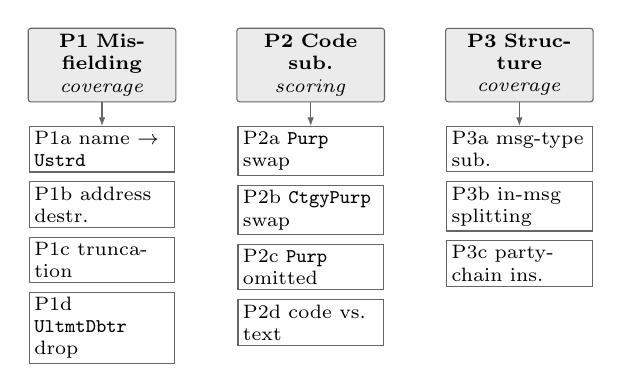
\begin{tikzpicture}[
  font=\scriptsize,
  fam/.style={draw,rounded corners=1pt,fill=black!8,inner sep=2.2pt,
              text width=1.72cm,align=center,minimum height=8mm},
  prim/.style={draw,inner sep=1.8pt,text width=1.72cm,align=left,
               minimum height=4.6mm},
  every path/.style={-{Latex[length=1.1mm]},draw=black!60}
]
\node[fam] (p1) at (0,0) {\textbf{P1 Misfielding}\\\emph{coverage}};
\node[fam] (p2) at (2.65,0) {\textbf{P2 Code sub.}\\\emph{scoring}};
\node[fam] (p3) at (5.3,0) {\textbf{P3 Structure}\\\emph{coverage}};

\node[prim,below=3.0mm of p1] (a1) {P1a name $\to$ \texttt{Ustrd}};
\node[prim,below=1.1mm of a1] (a2) {P1b address destr.};
\node[prim,below=1.1mm of a2] (a3) {P1c truncation};
\node[prim,below=1.1mm of a3] (a4) {P1d \texttt{UltmtDbtr} drop};

\node[prim,below=3.0mm of p2] (b1) {P2a \texttt{Purp} swap};
\node[prim,below=1.1mm of b1] (b2) {P2b \texttt{CtgyPurp} swap};
\node[prim,below=1.1mm of b2] (b3) {P2c \texttt{Purp} omitted};
\node[prim,below=1.1mm of b3] (b4) {P2d code vs.\ text};

\node[prim,below=3.0mm of p3] (c1) {P3a msg-type sub.};
\node[prim,below=1.1mm of c1] (c2) {P3b in-msg splitting};
\node[prim,below=1.1mm of c2] (c3) {P3c party-chain ins.};

\draw (p1) -- (a1); \draw (p2) -- (b1); \draw (p3) -- (c1);
\end{tikzpicture}
\caption{Evasion primitives for ISO~20022 credit transfers. Families are
labelled by the control property they attack: \emph{coverage} means the
screening engine never reads the content; \emph{scoring} means it reads the
content but is given a misleading prior. Conceptual diagram.}
\label{fig:taxonomy}
\end{figure}

%%=====================================================================
\section{Benchmark, Validation Framework and Detectors}
\label{sec:bench}
%%=====================================================================

\subsection{Validation constraints}
The framework states five constraint classes over a message $x$. They are
ordered from cheap and local to expensive and longitudinal, and each yields
features for the detectors.

\textbf{C1 Code-list and schema validity.} \texttt{Purp/Cd} is a member of
\texttt{ExternalPurpose1Code}; \texttt{Ctry} is a valid ISO~3166 alpha-2
code; the instance validates against the message schema.

\textbf{C2 Structural completeness.} The post-2026 minimum
(\texttt{TwnNm}, \texttt{Ctry}) is populated for every agent and
party~\cite{swift2026addr,cpmi2026}; \texttt{AdrLine} does not carry tokens
that pattern-match to a structured child, such as a postcode or a country
name.

\textbf{C3 Cross-field consistency.} The purpose code is plausible given the
creditor's industry classification and the corridor; \texttt{CtgyPurp} agrees
with the batch structure; \texttt{UltmtDbtr} is present when the initiating
party is a PSP.

\textbf{C4 Code--narrative agreement.} The remittance text is consistent with
the declared purpose code. We implement this as a similarity between the text
and a code description, thresholded per code.

\textbf{C5 Longitudinal consistency.} The purpose-code distribution for a
(debtor, creditor, corridor) triple is consistent with its own history. This
operationalises the pattern-divergence signal the Federal Reserve article
describes~\cite{frb2026}.

C1 and C2 are hard constraints and produce violations. C3--C5 are soft and
produce continuous features. A key property of the design is that C1--C2
violations are dominated by accidental error, while C3--C5 is where the
deliberate and accidental cases could plausibly separate.

\subsection{Generator}
The generator emits pain.001.001.09 and pacs.008.001.08 instances. Schema
validity is verified, not asserted: 20\,000 messages drawn from a measured
corpus, covering all eleven primitives and every accidental-defect mode,
validate without error against the ISO~20022 XSDs for both message
definitions. It is seeded and deterministic: the same configuration and seed
reproduce the same corpus byte-for-byte.

\emph{Population.} Debtor and creditor entities carry an industry
classification, a home country and a corridor membership, and each pair is
assigned a purpose-code profile conditioned on industry and corridor.

\emph{Benign stream.} Messages sample a purpose code from the pair's profile
and populate address and party elements completely. Accidental defects are
then injected at rate $\eta$, with a defect mix taken from the failure modes
that market-practice guidance reports: purpose content written into
remittance information, partially destructured addresses, and absent optional
codes~\cite{pmpg2024}. $\eta$ is a benchmark parameter, not a measurement; the
protocol sweeps it.

\emph{Illicit stream.} A fraction $\rho$ of payments involve a
watchlist-adjacent party or a high-scrutiny corridor. Without evasion these
are the payments the screening abstraction is meant to alert on.

\emph{Adversarial stream.} For each illicit payment an evader with budget
$k$ and knowledge $\kappa \in \{\text{black},\text{grey}\}$ solves
\eqref{eq:evader} against the abstraction $\pi$ below, by enumeration over
admissible primitive subsets. Ground truth records the primitive set
applied, its source and target elements, and $\pi$ before and after.

\emph{Screening abstraction.} $\pi$ is a published, parameterised model, not a
deployed engine: a name-matching component over the screened element set
$F_s$ with a fuzzy-match threshold, plus an additive risk score over purpose
code, corridor, amount band and party completeness, alerted at threshold
$\tau$ calibrated to a stated alert budget. Making $\pi$ explicit is what
makes the evasion metric reproducible, and is also its main limitation
(Section~\ref{sec:disc}).

Because $\mathrm{SEL}$ is a ratio of pass-through probabilities it is acutely
sensitive to the baseline $\pi_0$, so we solve for the parameters rather than
choose them. Given a target $\pi_0$ --- the mean alert probability over
\emph{un-evaded} illicit traffic --- we bisect the name-match probability
$p_{\mathrm{name}}$ and, where the score leg puts the target out of reach,
the threshold $\tau$, holding $\pi_{\mathrm{floor}}=0.10$. Targets $0.30$,
$0.45$ and $0.60$ solve to $(p_{\mathrm{name}},\tau) = (0.004,0.761)$,
$(0.004,0.623)$ and $(0.125,0.550)$. We report at $\pi_0=0.45$ and never
quote $\mathrm{SEL}$ without the sweep.

\subsection{Screening-evasion lift}
Detection accuracy alone does not say whether an attack was worth mounting.
Let $\pi_0$ be the alert probability for an illicit payment with no
manipulation and $\pi_m$ the alert probability after $m$. Define
\begin{equation}
\mathrm{SEL}(m) \;=\; \frac{1-\pi_m}{1-\pi_0},
\label{eq:sel}
\end{equation}
the multiplicative increase in the probability that an illicit payment passes
un-alerted. $\mathrm{SEL}=1$ means the manipulation bought the adversary
nothing. With a detector $D$ in place, the payment must evade both controls,
so we also report the residual lift
\begin{equation}
\mathrm{SEL_{res}}(m,D) \;=\;
\frac{(1-\pi_m)\,(1-\delta_m)}{(1-\pi_0)\,(1-\delta_0)},
\label{eq:selres}
\end{equation}
where $\delta$ is the detection rate of $D$ at the operating threshold. The
gap between \eqref{eq:sel} and \eqref{eq:selres} is the part of the attack the
detector actually removes, which is the quantity a control owner needs and is
not recoverable from a ROC curve. Both are reported with bootstrap intervals
over the corpus.

\subsection{Detectors}
Five configurations, from the weakest realistic control upward.
$D_0$ applies C1--C2 only, which is what schema and code-list validation give
for free. $D_1$ adds hand-set thresholds on C3--C4, a rule-based validator of
the kind a bank could deploy without a model. $D_2$ is a supervised
gradient-boosted classifier over raw field values --- one-hot purpose code, corridor,
amount band, completeness flags --- trained on gaming labels; it is the naive
baseline that assumes labels exist, which in production they largely do not.
$D_3$ is an isolation forest~\cite{liu2008} over the C3--C5 constraint
features, trained unsupervised on the benign stream only. $D_4$ combines
$D_1$ and $D_3$ by equal-weight rank averaging, not by summing $z$-scores:
$D_1$ is a small-support sum of violations and $D_3$ a continuous isolation
score, and standardising lets the heavier tail dominate (0.775 against 0.768
at $n=40\,000$). The comparison of interest is
$D_2$ against $D_3$: whether constraint features computed without labels match
a supervised model that needs them.

%%=====================================================================
\section{Evaluation Protocol}
\label{sec:proto}
%%=====================================================================

The protocol fixes what will be measured before anything is run.

\emph{Corpora.} A benign corpus and an adversarial corpus generated from the
same population and seeds, so that the only difference is the manipulation.
Every result below uses $n=200\,000$ messages per run across five corridors
at seeds 7, 8 and 9, with $\rho=0.05$ and $\eta=0.15$ unless swept. The
ablations and the $\eta$ sweep use $n=100\,000$, the calibration sweep
$n=50\,000$.

\emph{Evader parameters.} Cost weight $\lambda=0.18$, rationality
temperature $\mathrm{TEMP}=0.10$; neither is incidental. A perfectly
rational evader ($\mathrm{TEMP}=0$) concentrates on the cheapest primitive
and starves the per-primitive analysis, as does raising $\lambda$. The
softmax keeps all eleven populated, at no fewer than 399 instances each.

\emph{Primary metrics.} ROC-AUC for gaming detection; detection rate at
alert budgets of 1\% and 0.1\%; and $\mathrm{SEL}$, $\mathrm{SEL_{res}}$ per
primitive.

\emph{Ablations.} By primitive family; by evader budget $k \in \{1,2,3\}$;
by knowledge level $\kappa$; and by the accidental-defect rate $\eta$, swept
across a range bracketing plausible operational values. The $\eta$ sweep
answers the paper's question, measuring how fast separability degrades as
benign noise rises.

\emph{Leave-one-primitive-out.} Detectors that learn are trained with one
primitive family withheld and evaluated on it. Without this, a detector can
score well by learning the generator's own edit signature rather than the
property that makes the edit an attack. We treat the held-out result as the
headline number and the in-distribution result as an upper bound.

\emph{Reproducibility.} Configuration, seeds and library versions are
recorded per run; figures regenerate from the raw result files by released
scripts.

%%=====================================================================
\section{Results}
\label{sec:results}
%%=====================================================================

Every number here is measured. Seed spread never exceeds $0.012$ AUC.

\subsection{Hypotheses}
\emph{H1 is not confirmed as stated.} It predicted that coverage attacks
(P1 and P3) leave structural evidence and would already be caught by $D_1$.
The families behave nothing alike: against P1 alone $D_4$ reaches AUC
$0.855$, against P3 alone $0.519$, indistinguishable from chance
(Table~\ref{tab:ablation}). Grouping them was the error. Relocating a name
leaves a completeness signature; substituting the message type or inserting
an intermediary leaves a structurally ordinary message.

\emph{H2 is not confirmed, in either half.} It predicted that scoring attacks
(P2) leave no single-message evidence, so $D_1$ would fail on them and $D_3$
would not. $D_1$ does not fail: held out on P2 it scores $0.822$, its best family. Nor
does $D_3$ overtake it, at $0.796$. The premise was wrong --- a low-scrutiny
purpose code is implausible for the creditor's industry, which C3 sees, and
code--narrative decoupling is visible to C4, so the cross-message route
through C5 was never needed.

\emph{H3 is confirmed in its second clause only.} $\mathrm{SEL}$ is not
largest for P2a and P1a: at $\pi_0=0.45$ the structure family leads (P3b
$1.78$, P3a $1.77$, P3c $1.76$), P1a is fourth at $1.74$, and P2a is the
\emph{smallest} of the eleven at $1.45$ --- inverted. The second clause
holds, $\mathrm{SEL_{res}}$ falling furthest for P1a, $1.743$ to $1.650$.

\begin{figure}[!tbp]
\centering
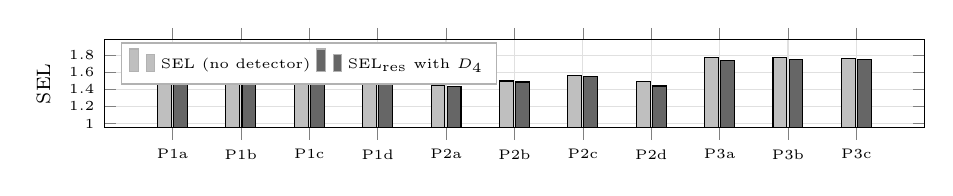
\begin{tikzpicture}
\begin{axis}[
  width=0.99\columnwidth, height=2.7cm,
  ybar=0.8pt, bar width=5pt,
  ylabel={SEL},
  symbolic x coords={P1a,P1b,P1c,P1d,P2a,P2b,P2c,P2d,P3a,P3b,P3c},
  xtick=data, ymin=0.95, ymax=1.98,
  grid=both, grid style={black!12},
  legend style={at={(0.02,0.97)},anchor=north west,font=\tiny,
                draw=black!30,legend columns=2},
  label style={font=\scriptsize}, tick label style={font=\tiny}
]
\addplot[fill=black!25] coordinates {(P1a,1.743) (P1b,1.653) (P1c,1.614) (P1d,1.652) (P2a,1.450) (P2b,1.498) (P2c,1.566) (P2d,1.487) (P3a,1.768) (P3b,1.776) (P3c,1.761)};
\addlegendentry{$\mathrm{SEL}$ (no detector)}
\addplot[fill=black!60] coordinates {(P1a,1.650) (P1b,1.589) (P1c,1.601) (P1d,1.584) (P2a,1.438) (P2b,1.486) (P2c,1.553) (P2d,1.439) (P3a,1.740) (P3b,1.745) (P3c,1.752)};
\addlegendentry{$\mathrm{SEL_{res}}$ with $D_4$}
\end{axis}
\end{tikzpicture}
\caption{Screening-evasion lift, seed 7, $\pi_0=0.45$; all eleven primitives clear
$n\!\ge\!30$ (399--5487), bootstrap half-widths $\pm0.021$ to $\pm0.075$.
The gap between the bars is what $D_4$ removes, and it is small. Mean lift
scales with the operating point: 1.40, 1.63, 1.80 at $\pi_0=0.30$, $0.45$,
$0.60$.}
\label{fig:sel}
\end{figure}

\begin{figure}[!tbp]
\centering
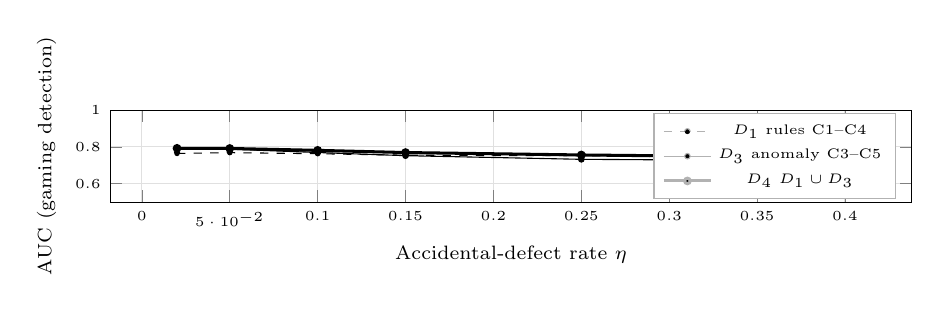
\begin{tikzpicture}
\begin{axis}[
  width=0.97\columnwidth, height=2.75cm,
  xlabel={Accidental-defect rate $\eta$}, ylabel={AUC (gaming detection)},
  ymin=0.5, ymax=1.0, grid=both, grid style={black!12},
  legend style={at={(0.98,0.97)},anchor=north east,font=\tiny,draw=black!30},
  label style={font=\scriptsize}, tick label style={font=\tiny}
]
\addplot[dashed,mark=*,mark size=1pt] coordinates {(0.020,0.7645) (0.050,0.7688) (0.100,0.7630) (0.150,0.7549) (0.250,0.7520) (0.400,0.7369)};
\addlegendentry{$D_1$ rules C1--C4}
\addplot[solid,mark=*,mark size=1pt] coordinates {(0.020,0.7927) (0.050,0.7876) (0.100,0.7695) (0.150,0.7523) (0.250,0.7325) (0.400,0.7237)};
\addlegendentry{$D_3$ anomaly C3--C5}
\addplot[solid,line width=1.1pt,mark=*,mark size=1pt] coordinates {(0.020,0.7923) (0.050,0.7915) (0.100,0.7812) (0.150,0.7693) (0.250,0.7561) (0.400,0.7418)};
\addlegendentry{$D_4$ $D_1 \cup D_3$}
\end{axis}
\end{tikzpicture}
\caption{The experiment the benchmark exists to run: AUC against the rate $\eta$ at
which \emph{benign} messages carry an accidental defect; $n=100\,000$ per
point, seed 7, $\pi_0=0.45$. Separability decays without collapsing ---
$D_4$ falls 0.792 to 0.742 across a twentyfold rise in $\eta$. $D_3$ learns
the benign distribution and is most noise-sensitive (0.793 to 0.724); $D_1$
is most stable (0.765 to 0.737), overtaking $D_3$ beyond $\eta\approx0.15$.}
\label{fig:eta}
\end{figure}

\begin{table}[!tbp]
\caption{Detector comparison. Mean over seeds 7--9, $n=200\,000$,
$\eta=0.15$, $\pi_0=0.45$.}
\label{tab:detectors}
\centering
\footnotesize
\begin{tabular}{@{}l@{\hspace{4pt}}c@{\hspace{4pt}}c@{\hspace{4pt}}c@{\hspace{4pt}}c@{\hspace{4pt}}c@{}}
\toprule
Detector & Lbl. & AUC & @1\% & @0.1\% & AUC$_\mathrm{LOO}$ \\
\midrule
$D_0$ schema/code list & no & 0.497 & 0.039 & 0.039 & 0.497 \\
$D_1$ rules C1--C4 & no & 0.756 & 0.095 & 0.042 & 0.767 \\
$D_2$ naive classifier & yes & 0.997 & 0.241 & 0.142 & 0.841 \\
$D_3$ anomaly C3--C5 & no & 0.749 & 0.017 & 0.005 & 0.769 \\
$D_4$ $D_1 \cup D_3$ & no & 0.767 & 0.021 & 0.007 & 0.784 \\
\bottomrule
\end{tabular}
\vspace{1pt}
\par\raggedright\scriptsize
Lbl.: needs gaming labels. @$p$: TPR at budget $p$. AUC$_\mathrm{LOO}$:
leave-one-primitive-family-out over the three families;
Section~\ref{sec:disc} states how far it is contaminated.
\end{table}

\begin{table}[!tbp]
\caption{Ablation. AUC and mean $\mathrm{SEL_{res}}$ for $D_4$,
$n=100\,000$, seed 7, $\pi_0=0.45$.}
\label{tab:ablation}
\centering
\footnotesize
\begin{tabular}{@{}llcc@{}}
\toprule
Factor & Setting & AUC & $\mathrm{SEL_{res}}$ \\
\midrule
Primitive family & P1 only & 0.855 & 1.27 \\
 & P2 only & 0.883 & 1.37 \\
 & P3 only & 0.519 & 1.88 \\
Evader budget & $k=1$ & 0.689 & 1.39 \\
 & $k=2$ & 0.769 & 1.61 \\
 & $k=3$ & 0.833 & 1.63 \\
Knowledge & black-box & 0.674 & 1.71 \\
 & grey-box & 0.769 & 1.61 \\
\bottomrule
\end{tabular}
\end{table}

\subsection{Detectors}
$D_0$ sits at chance: every manipulation leaves a schema-valid,
code-list-valid message, so validation alone sees nothing. The premise is
measured, not assumed. Among the label-free detectors $D_3$ does not
overtake $D_1$ in distribution and does so only marginally held out; $D_4$
leads the three. The comparison Section~\ref{sec:bench} set up resolves
against the constraint features --- $D_2$ leads on both columns --- so
labels still buy a great deal. At the budgets a screening operation occupies
it is worse: $D_4$ recovers $2.1\%$ of manipulated messages at a 1\% budget
and $0.7\%$ at $0.1\%$, below $D_1$'s $9.5\%$ and $4.2\%$. Nothing
label-free here is deployable.

\subsection{What would have falsified the approach}
Neither fired. P2 detection reaches AUC $0.883$ against a $D_0$ baseline of
$0.497$ at $\eta=0.15$, so the constraint features do separate deliberate
from accidental misfielding; and $\mathrm{SEL}$ spans $1.45$--$1.78$ at
$\pi_0=0.45$ and $1.23$--$2.19$ across the sweep, nowhere near 1, so the
abstraction is sensitive to the fields the adversary reaches. The
contribution survives; its size, not its existence, disappoints.

%%=====================================================================
\section{Discussion, Ethics and Threats to Validity}
\label{sec:disc}
%%=====================================================================

\subsection{Responsible framing}
Every primitive in Fig.~\ref{fig:taxonomy} is derivable from public
documents: the external code lists, the harmonised data
requirements~\cite{cpmi2026}, the guidance stating which element classes are
in scope~\cite{swiftgp2021}, and market-practice guidance recording
misfielding as a live problem~\cite{pmpg2024}. We publish no tuned
parameters against any deployed engine, and $\pi$ is a generic model rather
than a reproduction of any product. The intended use is control design: a
bank can read the taxonomy as a checklist of coverage gaps in its own
screened element set. We deliberately withhold corridor- and code-specific
weightings that would make the generator an operational recipe.

\subsection{Data and ethics}
The corpus is entirely synthetic. No real payment message, customer record
or employer data is used, and no proprietary information appears in the
generator or its configuration. Entities, accounts and names are drawn from
generated distributions, so the release carries no personal data and needs
no consent regime. Generator, seeds, configuration and harness are released
so others can reproduce or contest the results.

\subsection{Threats to validity}
\emph{Construct.} $\pi$ is an abstraction of screening, not a screening
engine. Every $\mathrm{SEL}$ value is therefore relative to a model whose
parameters we chose. A different weighting could reorder the primitives. This
is the most serious limitation in the paper, and it is not removed by any
mitigation available to us without access to a production engine.

\emph{Internal.} Two measured properties of the generator inflate Table~\ref{tab:detectors}.
The benign stream never batches --- every un-manipulated message has
$n_{\mathrm{splits}}=1$ while P3b sets it to 3--7, so
$n_{\mathrm{splits}}>1$ implies manipulation with precision $1.000$ and
covers $59.9\%$ of manipulated messages. $D_2$ exploits it and falls from
$0.997$ to $0.901$ when the feature is withheld; real pain.001 files batch
routinely, so this is a property of the code, not of payments. It flatters
no other detector: $D_1$ never reads it and $D_3$ cannot split on a feature
constant in training, which is also why P3 alone scores $0.519$. Second,
leave-one-primitive-family-out is contaminated at $k=2$, because a message
can carry two families and withholding one does not withhold its partner ---
$99.9\%$ of held-out P1 messages, $77.5\%$ of P3 and $64.1\%$ of P2 still
carry a primitive the detector trained on, which is why $D_2$ barely drops
on P1, to $0.991$. AUC$_\mathrm{LOO}$ is an optimistic bound; the clean
version needs $k=1$ and a weaker adversary with it.

\emph{External.} We do not know the real distribution of purpose codes by
corridor and industry, and we do not know the real rate of accidental
misfielding. $\eta$ and the code profiles are assumptions swept over a range,
not estimates. Results will not transfer to a bank's own traffic without
recalibration against that traffic.

\emph{Conclusion.} The protocol has been run, so the detector numbers are
measurements, not hypotheses --- but measurements on one generator. Three
seeds bound the sampling noise and 1000-resample bootstrap intervals bound
the SEL estimates; neither touches the two generator properties above, which
are why AUC$_\mathrm{LOO}$ and $D_2$ are upper bounds. Two of the three
hypotheses were not confirmed, which we read as the protocol having been
worth running.

\subsection{What we would do next}
In the order the results demand: give the benign stream a realistic batch-
size distribution and re-run, which removes the $n_{\mathrm{splits}}$
artifact and lowers every number in Table~\ref{tab:detectors}; repeat the
ablation at $k=1$ for an uncontaminated leave-one-out figure; then attack
the construct threat, since validating $\pi$ against an anonymised
distribution of alert outcomes from one institution, without moving message
data, would make the SEL numbers calibrated rather than model-relative.
Defensive cost stays open, and the false positives a bank would absorb to
close each coverage gap decide whether any of this is deployable.

%%=====================================================================
\section{Conclusion}
%%=====================================================================

Structured payment data makes screening better and gives the originator a
finer instrument for shaping what screening sees. The mandate arriving in
November 2026 settles the first half of that trade; the second half has been
described in industry guidance as an accident and not yet studied as a
choice. We have specified the manipulations available to a message
originator, a set of validation constraints over the fields they touch, a
synthetic benchmark that generates both accidental and deliberate versions of
the same defects, and a metric that separates detector credit from screening
credit. Manipulation does still look different from ordinary error at a realistic
noise rate. The interesting number is how little that is worth: a detector
needing no labels ranks manipulated messages above benign ones about three
times in four, and at a 1\% alert budget takes back almost none of what the
manipulation bought.

%%=====================================================================
\setlength{\IEEEbibitemsep}{0pt}
\begin{thebibliography}{99}
\scriptsize

\bibitem{swift2026addr}
Swift, ``Unstructured address data is being removed: are you ready?'' Swift
Standards, 2026. [Online]. Available:
\url{https://www.swift.com/standards/iso-20022/removal-unstructured-address}
(accessed Aug.~16, 2026).

\bibitem{cpmi2026}
Committee on Payments and Market Infrastructures, \emph{Harmonised ISO~20022
Data Requirements for Enhancing Cross-Border Payments}, Bank for
International Settlements, updated report, Feb.~2026.

\bibitem{frb2026}
Federal Reserve Financial Services, ``Harnessing the power of ISO~20022: why
the global payment standard matters for fraud mitigation,'' \emph{Fed360},
Apr.~15, 2026.

\bibitem{swiftgp2021}
Swift, ``Guiding principles for screening ISO~20022 payments messages,''
Oct.~2021; endorsed by the Wolfsberg Group, Nov.~2021.

\bibitem{wolfsberg2023}
The Wolfsberg Group, \emph{Payment Transparency Standards}, 2023.

\bibitem{pmpg2024}
Payments Market Practice Group, \emph{ISO~20022 Market Practice Guidance:
Regulatory Reporting, Purpose of Payment and Category Purpose}, v1.1,
Jul.~2024.

\bibitem{boe2021}
Bank of England, \emph{UK Recommended Purpose Code List}, RTGS Renewal
Programme, 2021.

\bibitem{altman2023}
E. Altman, J. Blanuša, L. von Niederhäusern, B. Egressy, A. Anghel, and
K. Atasu, ``Realistic synthetic financial transactions for anti-money
laundering models,'' in \emph{Adv. Neural Inf. Process. Syst. 36 (NeurIPS
2023), Datasets and Benchmarks Track}, 2023.

\bibitem{oztas2023}
B. Oztas, D. Cetinkaya, F. Adedoyin, M. Budka, H. Dogan, and G. Aksu,
``Enhancing anti-money laundering: development of a synthetic transaction
monitoring dataset,'' in \emph{Proc. IEEE Int. Conf. e-Business Eng.
(ICEBE)}, 2023, pp.~47--54, doi:10.1109/ICEBE59045.2023.00028.

\bibitem{wang2025}
Q. Wang, W.-T. Tsai, T. Shi, W. Tang, and B. Du, ``Hide and seek in
transaction networks: a multi-agent framework for simulating and detecting
money laundering activities,'' \emph{Complex \& Intelligent Systems},
vol.~11, art.~271, 2025, doi:10.1007/s40747-025-01913-w.

\bibitem{busson2023}
A. J. G. Busson \emph{et al.}, ``Hierarchical classification of financial
transactions through context-fusion of transformer-based embeddings and
taxonomy-aware attention layer,'' arXiv:2312.07730, 2023.

\bibitem{camacho2025}
J. Camacho and R. A. Rodríguez-Gómez, ``Data quality tools to enhance a
network anomaly detection benchmark,'' \emph{Data}, vol.~10, no.~3, art.~33,
2025, doi:10.3390/data10030033.

\bibitem{dalvi2004}
N. Dalvi, P. Domingos, Mausam, S. Sanghai, and D. Verma, ``Adversarial
classification,'' in \emph{Proc. 10th ACM SIGKDD Int. Conf. Knowl. Discovery
and Data Mining}, 2004, pp.~99--108.

\bibitem{bruckner2011}
M. Brückner and T. Scheffer, ``Stackelberg games for adversarial prediction
problems,'' in \emph{Proc. 17th ACM SIGKDD Int. Conf. Knowl. Discovery and
Data Mining}, 2011, pp.~547--555.

\bibitem{biggio2013}
B. Biggio \emph{et al.}, ``Evasion attacks against machine learning at test
time,'' in \emph{Proc. ECML PKDD}, 2013, pp.~387--402.

\bibitem{liu2008}
F. T. Liu, K. M. Ting, and Z.-H. Zhou, ``Isolation forest,'' in \emph{Proc.
8th IEEE Int. Conf. Data Mining (ICDM)}, 2008, pp.~413--422.

\end{thebibliography}

\end{document}
